\documentclass[a4paper,12pt]{article}

\usepackage{fancyhdr}
\usepackage{lastpage}
\usepackage{amsmath, amssymb, amsthm}
\usepackage{bm}
\usepackage{wrapfig}
\usepackage{braket}
\usepackage{mathtools}
\usepackage[noend, linesnumbered]{algorithm2e}
\SetKwComment{Comment}{$\triangleright$\ }{}
\RestyleAlgo{ruled}
\usepackage[skip=2pt]{parskip}  
\usepackage{tikz}
\usetikzlibrary{arrows.meta, positioning}
\usepackage[edges]{forest} % Para a árvore de busca
\usepackage{graphicx} % Para imagens
\usepackage{array}          
\usepackage{booktabs}       


% ---- PREENCHA ----
\newcommand{\Lista}{1}
\newcommand{\Nome}{Isis Ardisson Logullo}
\newcommand{\NUSP}{7577410}
% -----------------------------

\newcommand{\N}{\mathbb{N}}
\newcommand{\bigO}[1]{\ensuremath{\mathcal{O}(#1)}}

\pagestyle{fancy}
\fancyhf{}
\fancyhead[L]{\Nome}
\fancyhead[R]{NUSP \NUSP}
\fancyfoot[L]{Lista \Lista}
\fancyfoot[C]{MAC0417}
\fancyfoot[R]{Página \thepage\ de \pageref{LastPage}}

\begin{document}

\section*{Exercício 1 - Transformação de Expansão de Contraste}

Deduza uma função contínua $s = T(r)$ que satisfaça o gráfico de expansão de contraste (\textit{contrast stretching}), onde $k$ é o ponto de transição e $E$ controla a inclinação como ilustrada na figura abaixo.

\begin{figure}[h]
	\centering
	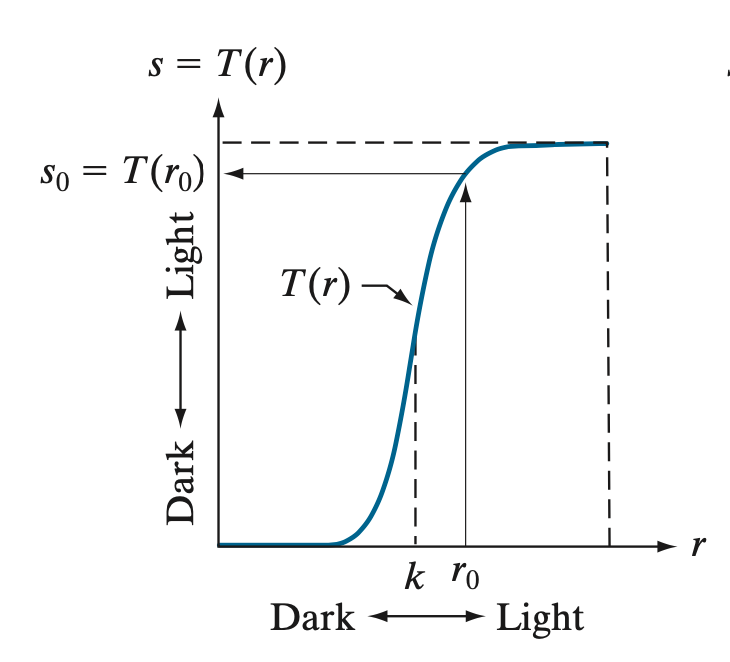
\includegraphics[width=0.7\linewidth]{screenshot001}
	\caption{}
	\label{fig:screenshot001}
\end{figure}

Note que além do parâmetro $k$, sua função deve incluir um parâmetro $E$ para controlar a inclinação da
função à medida que ela transiciona de valores de baixa intensidade para alta intensidade.\\

Sua função deve ser normalizada de modo que seus valores mínimo e máximo sejam 0 e 1, respectivamente.\\

\textbf{Dica}: Pense na conveniência de uma estrutura de fração onde o numerador é 1 e denominador é composto
por $1+f(r, k,E)$. Considere que $f$ é governada pela \textbf{competição} entre a intensidade do pixel $r$ e o ponto
crítico $k$. Pense em como a \textbf{razão} entre essas duas grandezas, quando potencializada pelo parâmetro
$E$, pode "empurrar" o resultado para os extremos 0 ou 1. Você deve definir $f$ para que $T(k) = 0,5$ e
$\lim_{r\to\infty} T(r) = 1$. Lembre-se de garantir a estabilidade para pixels pretos, ou seja, $\lim_{r\to0} T(r) = 0$.

\subsection*{Resposta:}

\bigskip

\begin{proof}

Sendo $1 / (1 + f(r, k, E))$ , e considerando que $f$ deve representar a "competição" entre a intensidade $r$ e o ponto $k$, podemos utilizar a razão entre essas grandezas.

A estrutura da função sigmoide é:

$$s = T(r) = \frac{1}{1 + \left(\frac{k}{r}\right)^E}$$

Para $r = k$:

$$T(k) = \frac{1}{1 + (k/k)^E} = \frac{1}{1 + 1^E} = \frac{1}{2} = 0.5 \quad$$\\

Limite quando $r \to 0$:

Se $r \to 0$, então $(k/r) \to \infty$. Como $E$ controla a inclinação (sendo positivo), $(k/r)^E \to \infty$.

$$T(r) = \frac{1}{1 + \infty} = 0 \quad$$\\

Limite quando $r \to \infty$:

Se $r \to \infty$, então $(k/r) \to 0$.

$$T(r) = \frac{1}{1 + 0} = 1 \quad$$\\

Logo a função de transformação de expansão de contraste é:


$$T(r) = \frac{1}{1 + \left(\frac{k}{r}\right)^E}$$\\

Aumentar o valor de $E$ torna a transição em torno de $k$ mais abrupta, enquanto valores menores de $E$ produzem uma transição mais suave.

\end{proof}

\newpage
\section*{Exercício 4 - Especificação de Histograma e Transformações de Intensidade}

Suponha que uma imagem possua valores de intensidade contínuos com uma função de densidade de
probabilidade (PDF) dada por $p_{r}(r) = \frac{2r}{(L-1)^2}$ para $0 \leq r \leq L-1$, e $p_{r}(r) = 0$ para outros valores de $r$.\\

(a) Encontre a função de transformação que mapeia os valores de intensidade de entrada $r$ nos valores
$s$ de uma imagem com histograma equalizado.\\

(b) Encontre a função de transformação que, quando aplicada às intensidades equalizadas $s$, produzirá
uma imagem cuja PDF de intensidade seja $p_{z}(z) = \frac{3z^2}{(L-1)^3}$ para $0 \leq z \leq L-1$, e $p_{z}(z) = 0$ para
outros valores de $z$.\\

(c) Expresse a função de transformação obtida em (b) diretamente em termos de $r$, as intensidades da
imagem de entrada original.


\subsection*{Resposta:}

\bigskip

\begin{proof}

(a)

Temos $p_{r}(r) = \frac{2r}{(L-1)^2}$ para $0 \leq r \leq L-1$.\\

Para encontrar a função de transformação de equalização, utilizamos a Função de Distribuição Acumulada (CDF) da imagem de entrada, 
logo:

$$s = T(r) = (L-1) \int_{0}^{r} p_{r}(w) dw$$

Substituindo a PDF dada:

$$s = (L-1) \int_{0}^{r} \frac{2w}{(L-1)^2} dw$$

$$s = \frac{L-1}{(L-1)^2} \int_{0}^{r} 2w \, dw = \frac{1}{L-1} \left[ w^2 \right]_0^r$$

Portanto:
$$s = \frac{r^2}{L-1}$$

\end{proof}

\begin{proof}

(b) 

Para $p_{z}(z) = \frac{3z^2}{(L-1)^3}$, calculamos a transformação de equalização teórica $H(z)$:\\


$$s = H(z) = (L-1) \int_{0}^{z} p_{z}(w) dw$$

$$s = (L-1) \int_{0}^{z} \frac{3w^2}{(L-1)^3} dw = \frac{L-1}{(L-1)^3} \int_{0}^{z} 3w^2 \, dw$$

$$s = \frac{1}{(L-1)^2} \left[ w^3 \right]_0^z = \frac{z^3}{(L-1)^2}$$

Para encontrar a função que transforma as intensidades equalizadas $s$ em $z$, isolamos $z$:


$$z^3 = s \cdot (L-1)^2$$

Logo: 

$$z = \sqrt[3]{s \cdot (L-1)^2}$$

\end{proof}

\begin{proof}

(c)

Para obter a transformação direta, substituímos a expressão de $s$ obtida no item (a) na função encontrada no item (b):\\

$$z = \sqrt[3]{\left( \frac{r^2}{L-1} \right) \cdot (L-1)^2}$$

$$z = \sqrt[3]{r^2 \cdot (L-1)}$$

Logo: 

$$z = [r^2(L-1)]^{1/3}$$

\end{proof}


\newpage
\section*{Exercício 6 - Transformação de Intensidade via Especificação Geométrica
	de PDF}

Uma imagem com intensidades no intervalo [0, 1] possui a função de densidade de probabilidade (PDF),
$p_{r}(r)$, mostrada na figura abaixo à esquerda.

\begin{figure}[h]
	\centering
	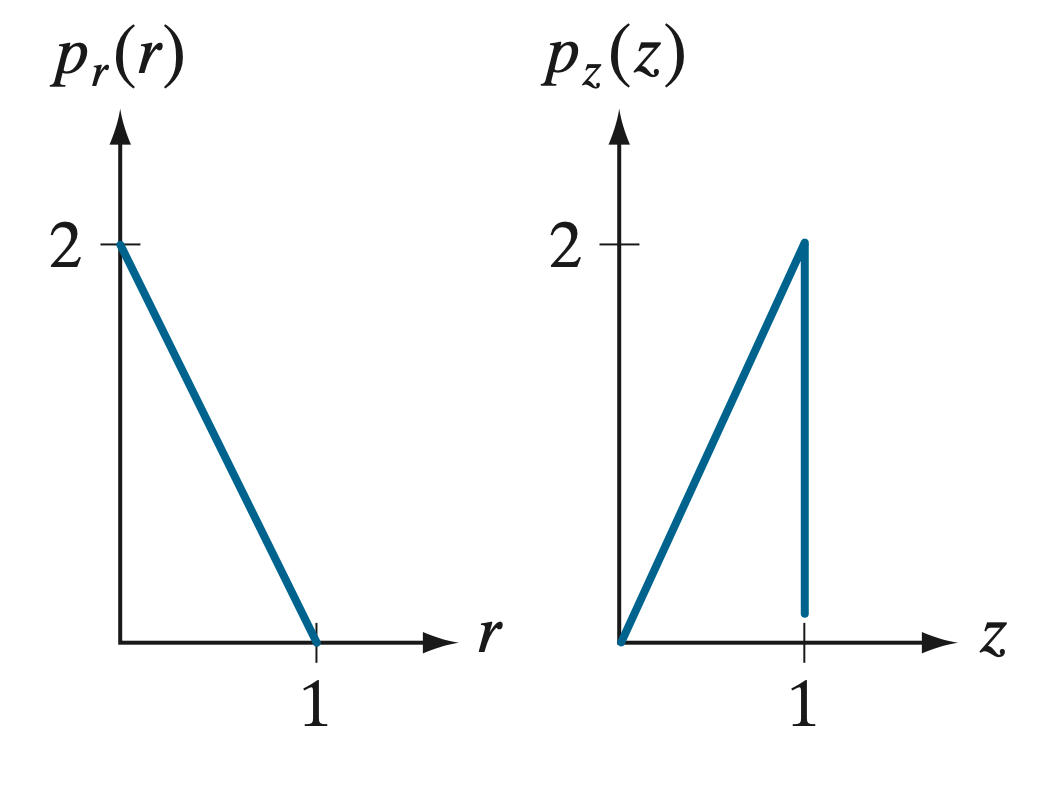
\includegraphics[width=0.7\linewidth]{screenshot002}
	\caption{}
	\label{fig:screenshot002}
\end{figure}

Deseja-se transformar os níveis de intensidade desta imagem para que eles passem a ter a PDF especificada,
$p_{z}(z)$, mostrada na figura à direita. Assumindo grandezas contínuas, encontre a função de
transformação (expressa em termos de $r$ e $z$) que realize esta operação.\\

\textbf{Dica}: Primeiro, determine as expressões analíticas para $p_{r}(r)$ e $p_{z}(z)$ no intervalo [0, 1] utilizando as
equações das retas apresentadas nos gráficos. Em seguida, utilize o método de especificação de histograma,
igualando as funções de distribuição acumulada (CDFs) para encontrar a relação direta entre $r$ e $z$.


\subsection*{Resposta:}

\bigskip

\begin{proof}

PDF da imagem original ($p_r(r)$): \\
É uma reta decrescente que passa pelos pontos $(0, 2)$ e $(1, 0)$.\\
A equação da reta é $y = ax + b$.\\
$b = 2$ (interseção com o eixo y).\\
Inclinação $a = \frac{0 - 2}{1 - 0} = -2$.\\
Logo, $p_r(r) = -2r + 2$ para $0 \leq r \leq 1$.\\

PDF especificada ($p_z(z)$): \\
É uma reta crescente que passa pelos pontos $(0, 0)$ e $(1, 2)$.\\
$b = 0$ (interseção com o eixo y).\\
Inclinação $a = \frac{2 - 0}{1 - 0} = 2$.\\
Logo, $p_z(z) = 2z$ para $0 \leq z \leq 1$.\\

Histograma no domínio contínuo igualando as CDFs de $r$ e $z$:\\
CDF de $r$ ($s = T(r)$):

$$s = \int_{0}^{r} p_r(w) dw = \int_{0}^{r} (-2w + 2) dw = \left[ -w^2 + 2w \right]_0^r$$

$s = -r^2 + 2r$\\

CDF de $z$ ($s = G(z)$):\\

$$s = \int_{0}^{z} p_z(w) dw = \int_{0}^{z} (2w) dw = \left[ w^2 \right]_0^z$$

$s = z^2$\\

Igualamos as duas expressões de $s$ para encontrar a relação direta entre as intensidades\\
$$z^2 = -r^2 + 2r$$

Assim temos: \\

$$z = \sqrt{2r - r^2}$$

\end{proof}

\newpage
\section*{Exercício 8 - Aplicação Prática da Equalização de Histograma}

Considere a distribuição de intensidade e os valores do histograma para uma imagem digital de 3 bits
com dimensões 64 × 64 pixels, conforme apresentados na tabela abaixo.

\begin{figure}[h]
	\centering
	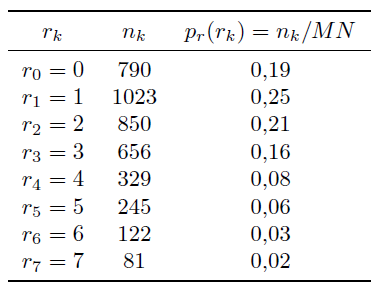
\includegraphics[width=0.7\linewidth]{screenshot003}
	\caption{}
	\label{fig:screenshot003}
\end{figure}

Determine (a) a função de transformação para a equalização do histograma e (b) apresente o histograma
equalizado resultante.


\subsection*{Resposta:}

\bigskip

A função de transformação para uma imagem digital é dada pela soma acumulada das probabilidades (CDF):


$$s_k = T(r_k) = (L-1) \sum_{j=0}^{k} p_r(r_j)$$\\


Como a imagem é de 3 bits, temos $L-1 = 7$. Os valores de $s_k$ devem ser arredondados para o inteiro mais próximo.\\

\begin{table}[h]
	\centering
	\caption{Processo de Equalização de Histograma para Imagem de 3 bits}
	\begin{tabular}{|c|c|c|c|c|}
		\hline
		$r_k$ & $p_r(r_k)$ & $\sum p_r(r_j)$ (Acumulado) & $7 \times \sum p_r(r_j)$ & $s_k$ (Arredondado) \\ \hline
		$r_0=0$ & 0,19 & 0,19 & 1,33 & 1 \\ \hline
		$r_1=1$ & 0,25 & 0,44 & 3,08 & 3 \\ \hline
		$r_2=2$ & 0,21 & 0,65 & 4,55 & 5 \\ \hline
		$r_3=3$ & 0,16 & 0,81 & 5,67 & 6 \\ \hline
		$r_4=4$ & 0,08 & 0,89 & 6,23 & 6 \\ \hline
		$r_5=5$ & 0,06 & 0,95 & 6,65 & 7 \\ \hline
		$r_6=6$ & 0,03 & 0,98 & 6,86 & 7 \\ \hline
		$r_7=7$ & 0,02 & 1,00 & 7,00 & 7 \\ \hline
	\end{tabular}
\end{table}

\newpage

Para obter o novo histograma $p_s(s_k)$, somamos as probabilidades originais $p_r(r_k)$ que foram mapeadas para o mesmo valor de saída $s_k$.\\

\begin{itemize}
	\item $s=1$: Vem apenas de $r_0 \rightarrow p_s(1) = 0,19$
	\item $s=3$: Vem apenas de $r_1 \rightarrow p_s(3) = 0,25$
	\item $s=5$: Vem apenas de $r_2 \rightarrow p_s(5) = 0,21$
	\item $s=6$: Vem de $r_3$ e $r_4 \rightarrow p_s(6) = 0,16 + 0,08 = \mathbf{0,24}$
	\item $s=7$: Vem de $r_5, r_6$ e $r_7 \rightarrow p_s(7) = 0,06 + 0,03 + 0,02 = \mathbf{0,11}$
\end{itemize}

\bigskip

Histograma Final:

\begin{table}[h]
	\centering
	\caption{Histograma Equalizado Resultante}
	\begin{tabular}{|c|c|c|}
		\hline
		$s_k$ & $p_s(s_k)$ & $n_s$ (Número de pixels approx.) \\ \hline
		0 & 0,00 & 0 \\ \hline
		1 & 0,19 & 778 \\ \hline
		2 & 0,00 & 0 \\ \hline
		3 & 0,25 & 1024 \\ \hline
		4 & 0,00 & 0 \\ \hline
		5 & 0,21 & 860 \\ \hline
		6 & 0,24 & 983 \\ \hline
		7 & 0,11 & 451 \\ \hline
	\end{tabular}
\end{table}

Observe que, conforme previsto na teoria para o domínio discreto, o histograma resultante não é perfeitamente uniforme, apresentando espaços vazios e agrupamento de níveis.


\newpage
\section*{Exercício 9 - Especificação de Histograma com Distribuição Alvo}

Considere a mesma imagem hipotética de 64 × 64 pixels do exercício anterior. Deseja-se transformar o
histograma dessa imagem para que ele passe a ter os valores especificados na tabela abaixo.

\begin{figure}[h]
	\centering
	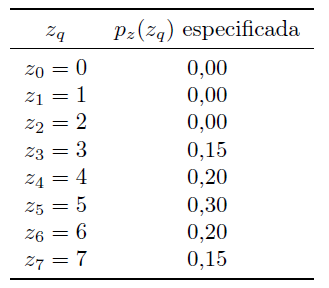
\includegraphics[width=0.7\linewidth]{screenshot004}
	\caption{}
	\label{fig:screenshot004}
\end{figure}

Obtenha a função de transformação necessária para realizar essa especificação de histograma.

\subsection*{Resposta:}

\bigskip
\setcounter{table}{0}

Equalização teórica para os níveis $z$ da PDF desejada para encontrar os valores $v_q$:\\

$v_q = \text{round}\left( 7 \cdot \sum_{j=0}^{q} p_z(z_j) \right)$\\

\begin{table}[h]
	\centering
	\caption{Equalização do Histograma Desejado ($v_q$)}
	\begin{tabular}{|c|c|c|c|c|}
		\hline
		$z_q$ & $p_z(z_q)$ & Soma Acumulada & $7 \times \text{Acum.}$ & $v_q$ (Arred.) \\ \hline
		$z_0=0$ & 0,00 & 0,00 & 0,00 & \textbf{0} \\ \hline
		$z_1=1$ & 0,00 & 0,00 & 0,00 & \textbf{0} \\ \hline
		$z_2=2$ & 0,00 & 0,00 & 0,00 & \textbf{0} \\ \hline
		$z_3=3$ & 0,15 & 0,15 & 1,05 & \textbf{1} \\ \hline
		$z_4=4$ & 0,20 & 0,35 & 2,45 & \textbf{2} \\ \hline
		$z_5=5$ & 0,30 & 0,65 & 4,55 & \textbf{5} \\ \hline
		$z_6=6$ & 0,20 & 0,85 & 5,95 & \textbf{6} \\ \hline
		$z_7=7$ & 0,15 & 1,00 & 7,00 & \textbf{7} \\ \hline
	\end{tabular}
\end{table}

\newpage

Para cada valor de $s_k$ obtido na imagem original, procuramos o valor de $v_q$ mais próximo. O nível $z_q$ correspondente será a nossa nova intensidade.

\begin{itemize}
	\item $s_k=1$: O $v_q$ mais próximo é $v_3=1$. Logo, $z=3$
	\item $s_k=3$: O $v_q$ mais próximo é $v_4=2$. Logo, $z=4$
	\item $s_k=5$: O $v_q$ mais próximo é $v_5=5$. Logo, $z=5$
	\item $s_k=6$: O $v_q$ mais próximo é $v_6=6$. Logo, $z=6$
	\item $s_k=7$: O $v_q$ mais próximo é $v_7=7$. Logo, $z=7$
\end{itemize}

\begin{table}[h]
	\centering
	\caption{Mapeamento Final para Especificação de Histograma}
	\begin{tabular}{|c|c|c|c|}
		\hline
		$r_k$ (Original) & $s_k$ (Equalizado) & $v_q \approx s_k$ & $z_q$ (Resultado) \\ \hline
		0 & 1 & $v_3=1$ & 3 \\ \hline
		1 & 3 & $v_4=2$ & 4 \\ \hline
		2 & 5 & $v_5=5$ & 5 \\ \hline
		3 & 6 & $v_6=6$ & 6 \\ \hline
		4 & 6 & $v_6=6$ & 6 \\ \hline
		5 & 7 & $v_7=7$ & 7 \\ \hline
		6 & 7 & $v_7=7$ & 7 \\ \hline
		7 & 7 & $v_7=7$ & 7 \\ \hline
	\end{tabular}
\end{table}


\newpage
\section*{Exercício 14 - Histogramas e Distribuição Espacial na Filtragem}

As duas imagens mostradas na figura a seguir são bastante diferentes, mas seus histogramas são iguais.

\begin{figure}[h]
	\centering
	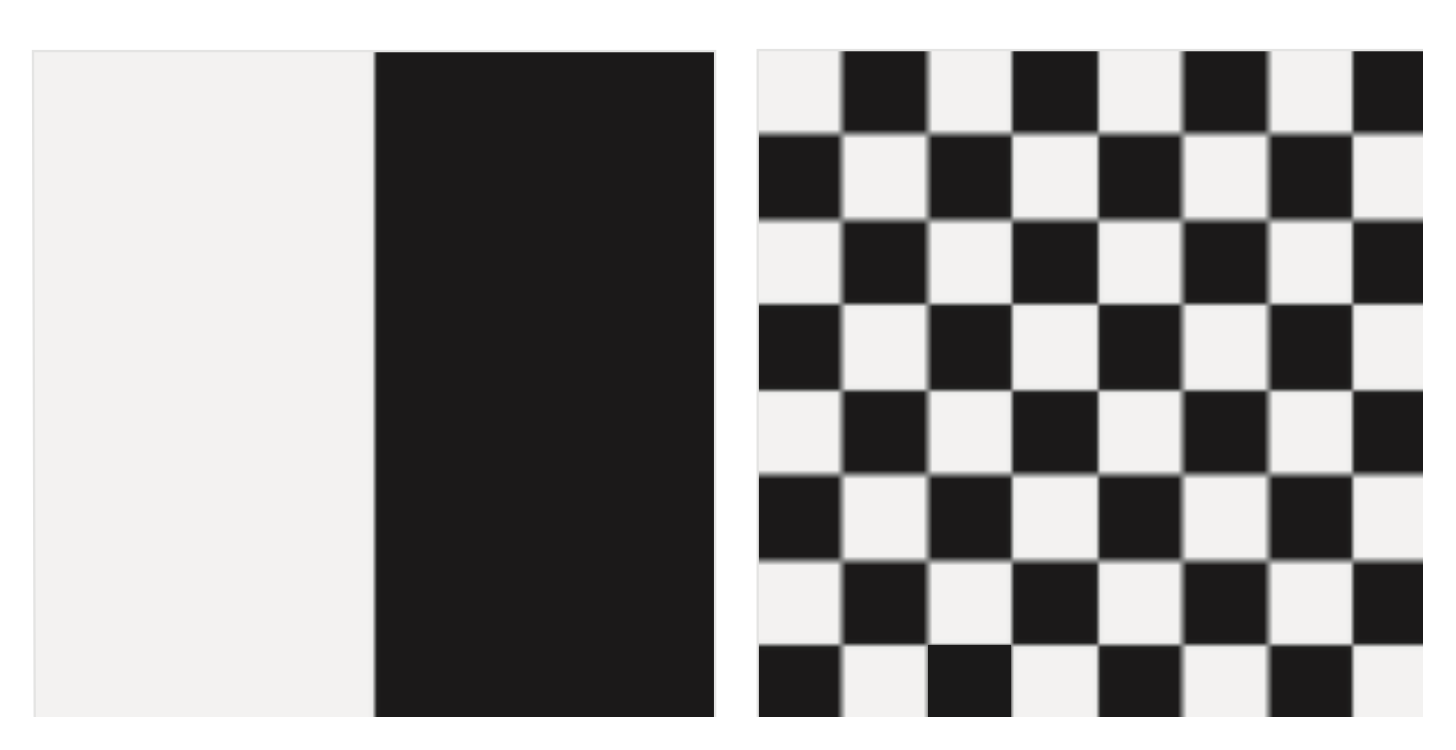
\includegraphics[width=0.7\linewidth]{screenshot005}
	\caption{}
	\label{fig:screenshot005}
\end{figure}

Considere que cada quadradrinho seja um pixel. Suponha que cada imagem seja suavizada (borrada)
utilizando um núcleo de média (\textit{box kernel}) de tamanho 3 × 3.\\

(a) Os histogramas das imagens suavizadas ainda seriam iguais? Explique.\\

(b) Se a sua resposta for não, esboce os dois histogramas ou apresente duas tabelas detalhando os
componentes dos histogramas.\\

\subsection*{Resposta:}

\bigskip

(a)  Não. A suavização é uma operação que depende da vizinhança espacial de cada pixel. O valor de um pixel na imagem suavizada é a média dos valores dos pixels cobertos pelo núcleo (kernel) de $3 \times 3$. Mesmo tendo a mesma contagem global de intensidades, a disposição espacial determina quais valores serão "misturados" pelo filtro. Em uma imagem onde pixels claros e escuros estão muito próximos, a média resultará em tons de cinza intermediários. Em uma imagem com grandes blocos uniformes, apenas as bordas desses blocos sofrerão alteração significativa, mantendo a maioria dos tons originais no histograma.\\


(b) 

Considere duas imagens de $6 \times 6$ pixels com intensidades 0 (preto) e 255 (branco):\\

Imagem A (Tabuleiro): Pixels 0 e 255 alternados.\\
Imagem B (Blocos): Metade esquerda 0, metade direita 255.\\

Histogramas Originais (Iguais): Ambos possuem 18 pixels com valor 0 e 18 pixels com valor 255.\\

Após Suavização $3 \times 3$:

Histograma de A: Como cada pixel está rodeado por vizinhos de intensidade oposta, quase todos os pixels resultarão em valores próximos à média (ex: cinza médio). O histograma apresentará um grande pico central.\\

Histograma de B: Os pixels no centro dos blocos (longe da divisória) permanecerão 0 ou 255, pois todos os seus vizinhos $3 \times 3$ têm o mesmo valor. Apenas os pixels na fronteira entre o preto e o branco assumirão valores intermediários. O histograma terá dois picos nas extremidades e poucos valores no centro.\\

A filtragem espacial destrói a igualdade dos histogramas porque ela processa a informação de contexto local, que é diferente em cada imagem.


\newpage
\section*{Exercício 15 - Conservação da Soma de Intensidades na Filtragem}

Uma imagem é filtrada com um núcleo (kernel) cujos coeficientes somam 1. Mostre que a soma dos
valores dos pixels nas imagens original e filtrada é a mesma.

\subsection*{Resposta:}

\bigskip

\begin{proof}

Seja $f(x, y)$ a imagem original e $w(s, t)$ o núcleo de filtragem (kernel). A imagem filtrada $g(x, y)$ é dada por:

$$g(x, y) = \sum_{s} \sum_{t} w(s, t) \cdot f(x-s, y-t)$$

Queremos mostrar que a soma de todos os pixels de $g$ é igual à soma de todos os pixels de $f$, ou seja:


$$\sum_{x} \sum_{y} g(x, y) = \sum_{x} \sum_{y} f(x, y)$$


$$\sum_{x} \sum_{y} g(x, y) = \sum_{x} \sum_{y} \left[ \sum_{s} \sum_{t} w(s, t) \cdot f(x-s, y-t) \right]$$


Como as somas são finitas, podemos reorganizar para somar primeiro sobre os índices do kernel ($s, t$):

$$\sum_{x} \sum_{y} g(x, y) = \sum_{s} \sum_{t} w(s, t) \left[ \sum_{x} \sum_{y} f(x-s, y-t) \right]$$


A expressão $\sum_{x} \sum_{y} f(x-s, y-t)$ representa a soma de todos os pixels da imagem original apenas deslocada espacialmente por $(s, t)$. Independentemente do deslocamento, a soma de todos os valores de $f$ é constante. Vamos chamá-la de $S_f$:

$$\sum_{x} \sum_{y} f(x-s, y-t) = S_f$$


$$\sum_{x} \sum_{y} g(x, y) = \sum_{s} \sum_{t} w(s, t) \cdot S_f$$


$$\sum_{x} \sum_{y} g(x, y) = S_f \cdot \left[ \sum_{s} \sum_{t} w(s, t) \right]$$


Temos: $\sum_{s} \sum_{t} w(s, t) = 1$.\\

Portanto:

$$\sum_{x} \sum_{y} g(x, y) = S_f \cdot (1) = S_f$$

Como a soma total dos pixels da imagem filtrada é igual à soma total dos pixels da imagem original ($S_f$), provamos que a operação de filtragem com um kernel de soma unitária preserva a intensidade média da imagem. 

\end{proof}


\newpage
\section*{Exercício 16 - Conservação da Nulidade na Filtragem}

Uma imagem é filtrada com um núcleo (kernel) cujos coeficientes somam 0. Mostre que a soma dos
valores dos pixels na imagem filtrada também é 0.


\subsection*{Resposta:}

\bigskip

\begin{proof}

Seja $f(x, y)$ a imagem original e $w(s, t)$ o núcleo de filtragem (kernel). A imagem filtrada resultante $g(x, y)$ é definida pela convolução:

$$g(x, y) = \sum_{s} \sum_{t} w(s, t) \cdot f(x-s, y-t)$$

Queremos mostrar que a soma de todos os pixels da imagem filtrada $g$ é zero, ou seja:


$$\sum_{x} \sum_{y} g(x, y) = 0$$


$$\sum_{x} \sum_{y} g(x, y) = \sum_{x} \sum_{y} \left[ \sum_{s} \sum_{t} w(s, t) \cdot f(x-s, y-t) \right]$$


Reorganizamos para processar primeiro a soma sobre a imagem original:

$$\sum_{x} \sum_{y} g(x, y) = \sum_{s} \sum_{t} w(s, t) \left[ \sum_{x} \sum_{y} f(x-s, y-t) \right]$$


A expressão $\sum_{x} \sum_{y} f(x-s, y-t)$ é a soma de todos os níveis de intensidade da imagem original $f$. Vamos chamar esse valor constante de $S_f$:


$$\sum_{x} \sum_{y} g(x, y) = \sum_{s} \sum_{t} w(s, t) \cdot S_f$$

Como $S_f$ não depende dos índices do kernel ($s, t$), podemos colocá-lo em evidência:


$$\sum_{x} \sum_{y} g(x, y) = S_f \cdot \left[ \sum_{s} \sum_{t} w(s, t) \right]$$

Temos: $\sum_{s} \sum_{t} w(s, t) = 0$.\\ 

Portanto:

$$\sum_{x} \sum_{y} g(x, y) = S_f \cdot 0 = 0$$


Provamos que, se a soma dos coeficientes do kernel é 0, a soma total dos pixels da imagem resultante será sempre 0.

\end{proof}


\newpage
\section*{Exercício 20 - Máscara de Realce de Nitidez em Passo Único}

Determine um núcleo (kernel) 3 × 3 que realize a operação de \textit{realce de nitidez} em uma única passagem
pela imagem. Assuma que a imagem suavizada $\bar{f}(x, y)$ é obtida através de um filtro de caixa (\textit{box filter})
de tamanho 3 × 3, conforme representado abaixo:

\begin{figure}[h]
	\centering
	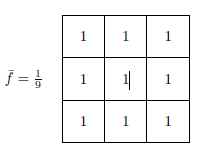
\includegraphics[width=0.7\linewidth]{screenshot006}
	\caption{}
	\label{fig:screenshot006}
\end{figure}

\textbf{Dica}: Utilize a definição $g(x, y) = f(x, y) + [f(x, y) - \bar{f}(x, y)]$ para combinar os filtros em uma única
matriz.

\subsection*{Resposta:}

\bigskip

\begin{proof}

O realce de nitidez é definido pela diferença entre a original e a suavizada:


$$g(x,y) = f(x,y) + [f(x,y) - \bar{f}(x,y)]$$


$$g(x,y) = 2f(x,y) - \bar{f}(x,y)$$


A imagem suavizada $\bar{f}(x,y)$ é obtida por um filtro $3\times3$:


$$\bar{f} = \frac{1}{9} \begin{bmatrix} 1 & 1 & 1 \\ 1 & 1 & 1 \\ 1 & 1 & 1 \end{bmatrix}$$


A imagem original $f(x,y)$, no contexto de kernels, pode ser representada por um impulso unitário (kernel identidade):


$$f = \begin{bmatrix} 0 & 0 & 0 \\ 0 & 1 & 0 \\ 0 & 0 & 0 \end{bmatrix}$$


$$g = 2 \begin{bmatrix} 0 & 0 & 0 \\ 0 & 1 & 0 \\ 0 & 0 & 0 \end{bmatrix} - \frac{1}{9} \begin{bmatrix} 1 & 1 & 1 \\ 1 & 1 & 1 \\ 1 & 1 & 1 \end{bmatrix}$$

$$g = \begin{bmatrix} 0 & 0 & 0 \\ 0 & 2 & 0 \\ 0 & 0 & 0 \end{bmatrix} - \begin{bmatrix} 1/9 & 1/9 & 1/9 \\ 1/9 & 1/9 & 1/9 \\ 1/9 & 1/9 & 1/9 \end{bmatrix}$$


$$g = \frac{1}{9} \left( \begin{bmatrix} 0 & 0 & 0 \\ 0 & 18 & 0 \\ 0 & 0 & 0 \end{bmatrix} - \begin{bmatrix} 1 & 1 & 1 \\ 1 & 1 & 1 \\ 1 & 1 & 1 \end{bmatrix} \right)$$


O núcleo $3\times3$ resultante que realiza o realce num único passo é:


$$g = \frac{1}{9} \begin{bmatrix} -1 & -1 & -1 \\ -1 & 17 & -1 \\ -1 & -1 & -1 \end{bmatrix}$$

Este kernel atua como um filtro de nitidez de alta frequência, onde o peso central elevado mantém a estrutura da imagem enquanto os pesos negativos circundantes subtraem as componentes suavizadas, realçando as bordas e detalhes finos.

\end{proof}

\end{document}
